%%%%%%%%%%%%%%%%%%%%%%%%%%%%%%%%%%%%%%%%%
% Focus Beamer Presentation
% LaTeX Template
% Version 1.0 (8/8/18)
%
% This template has been downloaded from:
% http://www.LaTeXTemplates.com
%
% Original author:
% Pasquale Africa (https://github.com/elauksap/focus-beamertheme) with modifications by 
% Vel (vel@LaTeXTemplates.com)
%
% Template license:
% GNU GPL v3.0 License
%
% Important note:
% The bibliography/references need to be compiled with bibtex.
%
%%%%%%%%%%%%%%%%%%%%%%%%%%%%%%%%%%%%%%%%%

%----------------------------------------------------------------------------------------
%	PACKAGES AND OTHER DOCUMENT CONFIGURATIONS
%----------------------------------------------------------------------------------------

\documentclass[handout]{beamer}

\usetheme{focus} % Use the Focus theme supplied with the template
% Add option [numbering=none] to disable the footer progress bar
% Add option [numbering=fullbar] to show the footer progress bar as always full with a slide countx


\definecolor{main}{RGB}{55, 135, 177}
\definecolor{text}{RGB}{60, 60, 80}
\definecolor{background}{RGB}{255, 255, 255}

\setbeamercovered{transparent}

%------------------------------------------------

\usepackage{booktabs} % Required for better table rules
\usepackage{tikz}
\usepackage{xepersian}
\settextfont{Vazir}
\setsansfont{FreeSerif}
\renewcommand{\baselinestretch}{1.3}

\title{\rl{ناتمامیت}}

\subtitle{\rl{سرگذشت یک قضیه‌ی دوران‌ساز}}

\author{\rl{مجید علی‌زاده}}

\titlegraphic{
\includegraphics[scale=.21]{images/tu-logo-hckd.png}}

\institute{\rl{	دانشکده‌ی ریاضی، آمار و علومِ کامپیوتر \\ دانشگاهِ تهران}}

\date{\rl{دی ۱۴۰۱}}


\begin{document}


\begin{frame}
	\maketitle
\end{frame}

\begin{frame}{\rl{کِرت گُدِل}}
	\begin{columns}[onlytextwidth]
		\column{0.6\textwidth}
		\flushleft
		\rl{در سال ۱۹۳۱، یک جوان ۲۵ ساله به نام «کرت گدل» یک مقاله در حوزه‌ی منطق ریاضی به نام چاپ کرد که شامل برهان دو قضیه‌ی مهم به نام «ناتمامیت» بود. این قضایا می‌گویند:
		برای هر نظام سازگار اصل-بنیاد که توانایی بیان حقایق حساب پایه را داشته باشد\\
		۱- گزاره‌هایی هستند که در این نظام اثبات‌پذیر نیستند، و\\
		۲- سازگاری این نظام در خودش اثبات‌پذیر نیست.}
		\column{0.4\textwidth}
		\flushright
		\rl{
		\begin{flushright}
			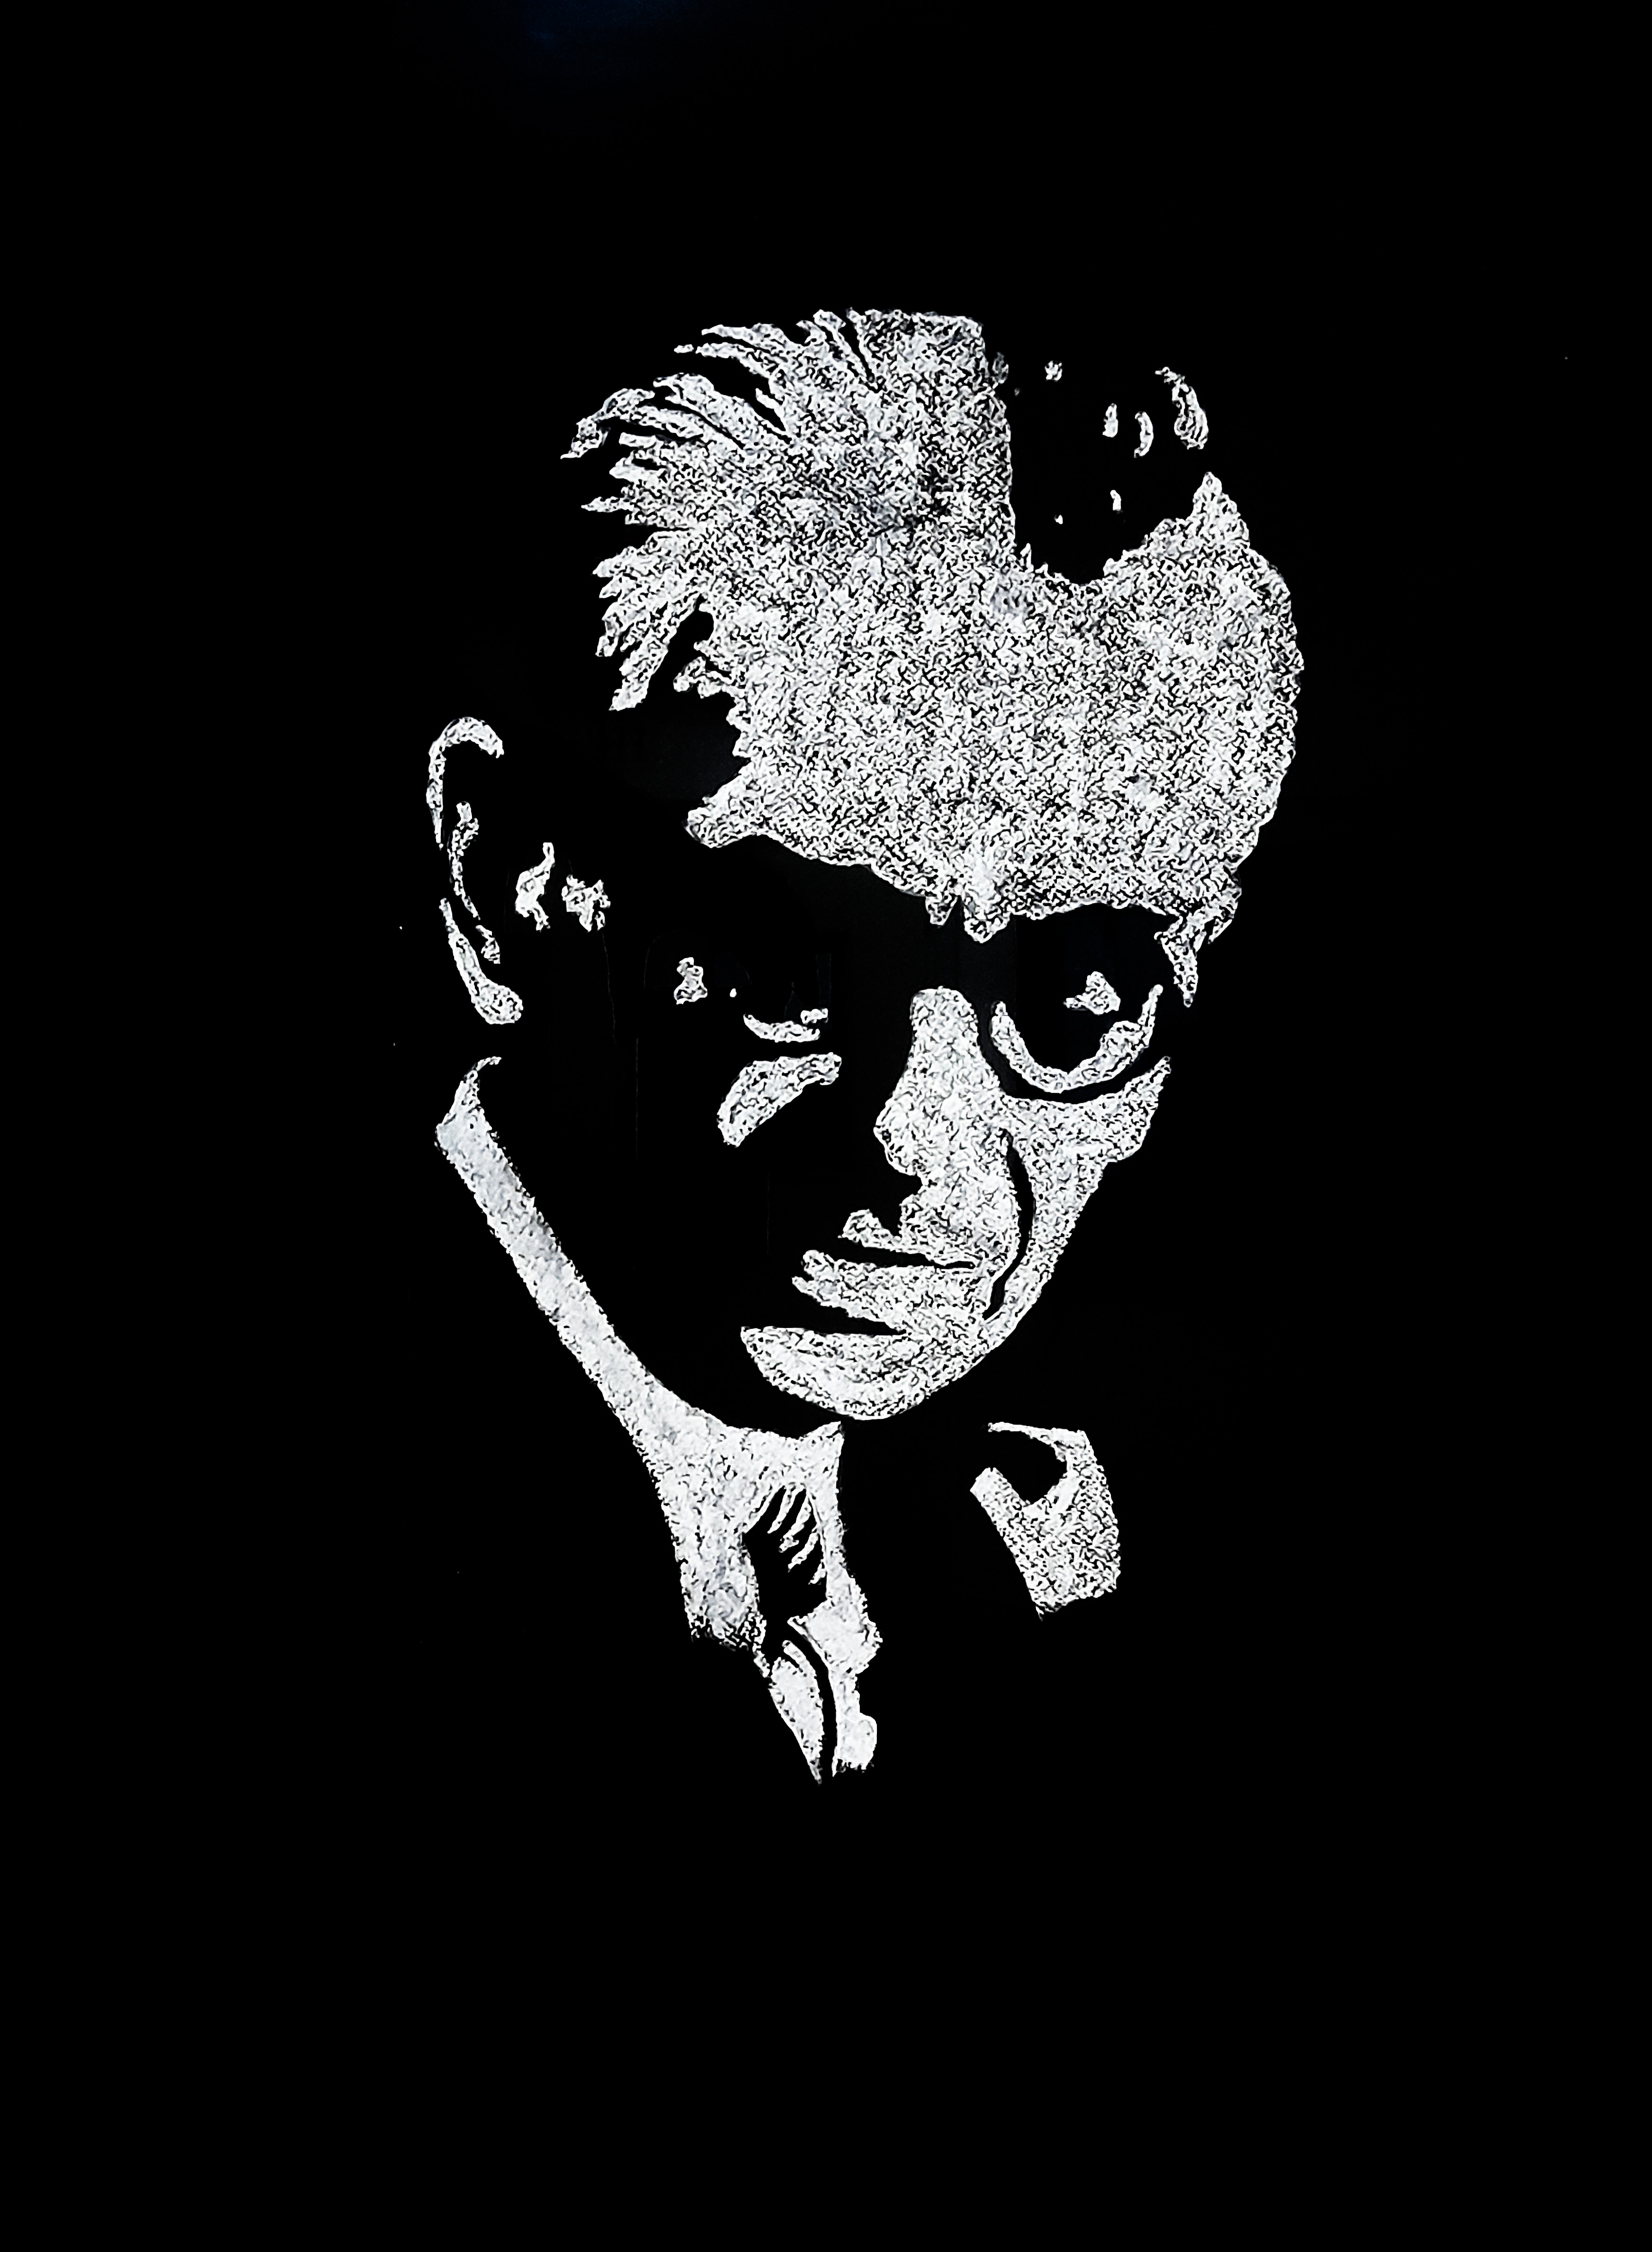
\includegraphics[width=\linewidth]{images/godel.jpg}
		\end{flushright}
		}
	\end{columns}
\end{frame}

\section{\rl{چکیده‌ای از تاریخ منطق}}

\begin{frame}{\rl{ارسطو}}
	\begin{flushright}
		\rl{مطالعه‌ی منطق اساساً با ارسطو شروع شده است. (۳۸۴ - ۳۲۲ ق.م.)
		} \vspace{1em}
	\end{flushright}
		\pause

		\rl{
			\lr{Posterior Analytics}\\
			\lr{Prior Analytics}\\
			\lr{Categories}\\
		} \vspace{1em}

		\pause
	\begin{flushright}
		\rl{تألیفات ارسطو شامل مطالعه‌ی نظام‌مند اصول استدلال علمی است که Syllogism نام گرفت. Syllogism، به جز در موارد پایه‌ای استدلال ریاضی، بسیار محدود است.}
	\end{flushright}
\end{frame}

\begin{frame}{\rl{دیگران}}
	\begin{flushright}
		\rl{در طی قرون وسطی، منطق ارسطو بر فلسفه سیطره داشت. تا جایی که امانوئل کانت، در اواخر قرن هجدهم چنین گفت: "منطق ارسطو کامل است و نیازی به بازنگری ندارد."
		} \vspace{1em} \vspace{1em}

		\pause

		\rl{یک قرن قبل از کانت، لایب‌نیتس تصور یک «حساب کامل» را در سر می‌پروراند و توانست گام‌های ابتدایی برای طراحی نظامی را بردارد که امروز به آن «منطق گزاره‌ها» می‌گوییم.
		} \vspace{1em}

		\pause

		\rl{قرن نوزدهم نقطه‌ی عطفی برای منطق بود.} \vspace{1em}
	\end{flushright}
\end{frame}


\begin{frame}{\rl{قرن نوزدهم}}
	\begin{flushright}
		\rl{در ۱۸۵۴ جورج بول کتاب The Laws of Thought را با نگاه جبری به منطق گزاره‌ها نوشت.} \vspace{1em}

		\pause

		\rl{در ۱۸۷۹ گوتلوب فرگه کتاب Concept-script (مفهوم-نگاشت) را نوشت که منطق گزاره‌ها را با سورها و رابطه‌ها، به مرتبه‌ای بالاتر گسترش داد که امروز به آن منطق مرتبه‌ی اوّل می‌گوییم.
		} \vspace{1em}

		\pause

		\rl{تفاوت نگاه بول و فرگه:\\
		بول: منطق به عنوان بخشی از ریاضیات\\
		فرگه: کاهش ریاضیات (حساب) به منطق
	 } \vspace{1em}
	\end{flushright}
\end{frame}


\begin{frame}{\rl{قرن نوزدهم}}
	\begin{flushright}
		\rl{ فرگه در کتاب \lr{Basic Laws of Arithmetic} نشان داد که چگونه می‌توان کل حقایق حساب را مطلقاً با مفروضات (بدیهیات) منطقی به دست آورد.} \vspace{1em}

		\pause

		\rl{ همان طور که خواهیم دید، این کار فرگه با پیدا شدن یک پارادوکس دچار مشکل شد. با این حال می‌توان او را خالق منطق جدید دانست.} \vspace{1em}

		\pause
		\rl{ ایده‌ی فرگه این بود که ریاضیات را می‌توان به منطق کاهش داد. به ویژه، فرگه امید داشت نشان دهد که صدق ریاضی، صدق پیشینی تحلیلی \lr{(A priori analytic truth)} است.} \vspace{1em}

		\pause
		\rl{جورج کانتور داستان را عوض کرد. او توانست بی‌نهایت را به عنوان یک شیء وارد ریاضیات کند.}
	\end{flushright}
\end{frame}


\begin{frame}{\rl{قرن بیستم: دوره‌ی عجیب}}
	\begin{flushright}
		\rl{برنامه‌ی کاهش تمام ریاضیات به منطق:\\
		$\bullet$ برنامه‌ی ریاضیات ساختی براوئر، بر پایه‌ی ساختمان ذهنی شهودی برای بازسازی ریاضیات\\
		$\bullet$ برنامه‌ی هیلبرت که روش انتزاعی‌ای که توسط کانتور و ددکیند معرفی شده بود را حمایت می‌کرد.
		}
	\end{flushright}
\end{frame}


\begin{frame}{\rl{برنامه‌ی هیلبرت}}
	\begin{flushright}
		\rl{طرح هیلبرت البته کاهش ریاضی به منطق نبود، بلکه بر آن بود که منطق و علم حساب باید با هم گسترش یابند تا در نتیجه کل نظام (ریاضی) عاری از ناسازگاری شود.\\
		این طرح و این ایمان هیلبرت برای نگاه اصل-بنیاد به ریاضی در مقاله‌ی ۱۹۲۲ کامل‌تر و به تفصیل بررسی شد.
		}\vspace{1em}

		\pause
		\rl{در مقاله‌ای در سال ۱۹۰۴ که درباره‌ی مبانی منطق و ریاضیات بود، برنامه‌ی فوق را پیشنهاد داد تا بتواند با نظام‌مندسازی منطق، حساب، آنالیز و نظریه‌ی مجموعه‌ها، آن‌ها را از شر پارادوکس‌ها رهایی بخشد.}
	\end{flushright}
\end{frame}

\section{\rl{صوری‌سازی ریاضیات}}


\begin{frame}{\rl{منظور از نظام اصل-بنیاد و روش صوری چیست؟}}
	\begin{flushright}
		\vspace{-1cm}
		\rl{\begin{block}{نظام اصل-بنیاد \lr{(Axiomatic System)}}
			یک نظام اصل-بنیاد مجموعه‌ای از گزاره‌ها (یا حقایق) است که در یک زبان صوری بیان می‌شود. این حقایق را «اصول» \lr{(Axiom)} نظام می‌نامند که صدق‌شان را بدون اثبات می‌پذیریم.\\ \vspace{1em}
			\pause
			در کنار اصول، مجموعه‌ای شامل «قواعد استنتاج» هم در نظام وجود دارند.
			با اعمال این قواعد روی اصول، گزاره‌های جدیدی «قضایا» \lr{(Theorem)} استنتاج می‌شود.
		\end{block}}
		\pause
		\rl{به عبارتی، اصول مجهز به قواعد هستند و استفاده از قواعد استنتاج، یعنی جایگزینی گزاره‌ها با گزاره‌های خاص دیگر.}
	\end{flushright}
\end{frame}

\begin{frame}{\rl{منظور از نظام اصل-بنیاد و روش صوری چیست؟}}
	\begin{flushright}
		\vspace{-1cm}
		\rl{\begin{block}{نظام اصل-بنیاد}
			\begin{itemize}
				\item[] اصول: مجموعه‌ای بدیهی از گزاره‌های صادق
    		\item[] قواعد: دستورالعملی برای ساخت گزاره‌های صادق بیشتر
			\end{itemize}
		\end{block}}
		\pause
		\rl{اصول و قواعد به گونه‌ای انتخاب می‌شوند که با شهود ما سازگار باشند، یا به عبارت دیگر، صدق آن‌ها بدیهی باشد.} \vspace{1em}

		\pause
		\rl{با اعمال متوالی قواعد استنتاج، که منجر به یک گزاره‌ی جدید می‌شود، می‌توان صدق این گزاره‌ی جدید را، که می‌تواند بسیار پیچیده و نابدیهی باشد، بدون رجوع دوباره به شهود پذیرفت.}
	\end{flushright}
\end{frame}

\begin{frame}[t]{\rl{مثالی از یک نظام اصل-بنیاد: هندسه‌ی اقلیدسی}}
	\vspace{-1cm}
	\begin{columns}[onlytextwidth]
		\column{0.4\textwidth}
		\flushleft
		\rl{هندسه‌ی اقلیدسی توسط فیلسوف یونانی ۳۰۰ سال قبل از میلاد معرفی شده و دارای ۵ اصل در مورد نقطه، خط و دایره است.}
		\column{0.6\textwidth}
		\flushright
		\rl{
		\begin{flushright} \emph{اصول}\\
				۱. از هر دو نقطه‌ی متمایز دقیقاً یک خط می‌گذرد.\\
				۲. هر دو خط متمایز حداکثر در یک نقطه یکدیگر را قطع می‌کنند.\\
				۳. یک دایره به هر مرکز و هر شعاع می‌توان رسم کرد.\\
				۴. همه‌ی زوایای قائمه برابر اند.\\
				۵. از یک نقطه خارج از یک خط تنها یک خط موازی با آن می‌گذرد.
		\end{flushright}
		}
	\end{columns}
\end{frame}

\begin{frame}[t]{\rl{مثالی از یک نظام اصل-بنیاد: هندسه‌ی اقلیدسی}}
	\vspace{-1cm}
	\begin{columns}[onlytextwidth]
		\column{0.4\textwidth}
		\flushleft
		\rl{هندسه‌ی اقلیدسی توسط فیلسوف یونانی ۳۰۰ سال قبل از میلاد معرفی شده و دارای ۵ اصل در مورد نقطه، خط و دایره است.}
		\column{0.6\textwidth}
		\flushright
		\rl{
		\begin{flushright} \emph{بدیهیات منطقی}\\
				‍۱. دو چیز که با یک چیز برابر باشند، با یکدیگر برابر اند.\\
				۲. اگر به دو چیز برابر، دو چیز برابر افزوده شوند، حاصل دو طرف برابر است.\\
				۳. اگر از دو چیز برابر، دو چیز برابر کاسته شوند، حاصل دو طرف برابر است.\\
				۴. اگر دو چیز بر هم منطبق باشند، با یکدیگر برابر اند.\\
				۵. کل از جزء بزرگ‌تر است.\\
		\end{flushright}
		}
	\end{columns}
\end{frame}

\begin{frame}{\rl{مثالی از یک نظام اصل-بنیاد: هندسه‌ی اقلیدسی}}
	\rl{اقلیدس توانست ۴۸ قضیه (غیر بدیهی) را، فقط با استنتاج منطقی و بدون توسل به شهود و ادراک هندسی، از این اصول به دست بیاورد.}\\ \vspace{1em}
	\pause
	\rl{اسپینوزا درباره‌ی مذهب و اخلاق به روش اصل‌بندی اقلیدس بحث کرد.}
\end{frame}

\begin{frame}{\rl{مشکل پارادوکس‌ها}}
	\begin{flushright}
		\rl{تا اواخر قرن نوزدهم، هندسه تنها شاخه‌ی «اصل‌بنیاد» ریاضی بود.} \vspace{1em}

		\pause
		\rl{کار ریاضی‌دانان در حوزه‌های دیگر ریاضی کمابیش بر درجه‌ی بالایی از بینش شهودی متکی بود.} \vspace{1em}

		\pause
		\rl{آن‌ها بدون داشتن یک مجموعه‌ی دقیق از اصول و بدون مشخص کردم دقیق این‌که چه نوع استنتاج‌هایی مجاز است، کارشان را پیش می‌بردند. (شاید چون نیازی به انجام این کار نمی‌دیدند.)} \vspace{1em}

		\pause
		\rl{داستان با کشف پارادوکس‌های گوناگون در اواخر قرن نوزدهم تغییر کرد.}
	\end{flushright}
\end{frame}

\begin{frame}{\rl{مشکل پارادوکس‌ها}}
	\begin{flushright}
		\rl{در آغاز قرن بیستم، جامعه‌ی ریاضی به خاطر ظهور پارادوکس‌هایی که اعتماد به شهود ریاضی را زیر سؤال می‌برد، با بحرانی در مبانی موجه شد.} \vspace{1em}

		\pause
		\rl{در سال ۱۹۰۱ برتراند راسل یک نقص در نظریه‌ی مجموعه‌ها (کانتور) پیدا کرد.} \vspace{1em}

		\[ R = \{x \mid x \not \in x\} \]

		\pause
		\rl{کانتور در نظریه‌اش هر خانواده‌ی قابل تعریف از اشیاء متمایز را مجموعه می‌دانست. بنابراین طبق نظریه‌ی کانتور، R یک مجموعه‌ی معتبر است.} \vspace{1em}
	\end{flushright}
\end{frame}

\begin{frame}{\rl{مشکل پارادوکس‌ها}}
	\begin{flushright}
		\rl{پارادوکس موقعی پیش می‌آید که بپرسیم «آیا R متعلق به خودش است؟»} \vspace{1em}

		\[ R \in R \iff R \not \in R \]

		\pause
		\rl{این پارادوکس نشان داد که مفهوم مجموعه‌ای که کانتور تعریف کرد مشکلی دارد، هر چند از نظر شهودی واقعاً معقول و پذیرفتنی است.}
	\end{flushright}
\end{frame}

\begin{frame}{\rl{صورت‌گرایی}}
	\begin{flushright}
		\rl{
			پارادوکس‌هایی از این دست باعث شد که ریاضی‌دان‌ها به فکر بیافتند که شهود به تنهایی راهنمای مطمئنی نیست، در نتیجه احساس نیاز به ارائه‌ی یک نظام اصل-بنیاد در این حوزه در اذهان ریاضی‌دانان بارور شد.
			دیدگاهی که بعدها نام صورت‌گرایی، یا formalism در ریاضیات به خود گرفت.
		} \vspace{1em}


		\pause
		\rl{
			با گذشت زمان حوزه‌های بیشتری با این دید مطالعه شدند. 
			برای نمونه: نظریه‌ی مجموعه‌های زرملو-فرانکل (ZF).
		}
	\end{flushright}
\end{frame}

\section{\rl{برنامه‌ی هیلبرت}}


\begin{frame}{\rl{برنامه‌ی هیلبرت}}
	\begin{flushright}
		\rl{هیلبرت راهی را پیشنهاد داد که فقط یک کیک داشته باشیم برای این که در عصرانه با هم بخوریم!\\
		۱- روش‌های کلاسیک را با اصول و قواعد صوری بیان کنیم (نمایش دهیم)؛ مسائل ریاضی را به عنوان یک گزاره در یک نظام اصل-بنیاد نمایش دهیم.\\
		۲- از یک روش «کران‌مند» (finitery) برای اثبات سازگاری این نظام‌های استنتاج صوری استفاده کنیم.
		} \vspace{1em}

		\pause
		\rl{		"روش اصل-بنیاد اکنون و برای هر زمانی، ابزار متناسب با ذهن بشری و لازم برای هر پژوهش دقیقی است. زمینه‌اش هر چه باشد، این روش منطقاً خدشه‌ناپذیر و در عین حال ثمربخش است، و نیز بیشترین آزادی حرکت را برای پژوهشگر حفظ می‌کند."
		}
	\end{flushright}
\end{frame}

\begin{frame}{\rl{برنامه‌ی هیلبرت}}
	\begin{flushright}
		\rl{هیلبرت خود نظام یک اصل-بنیاد برای حساب و آنالیز معرفی کرد.
		زرملو و فرانکل (اسکولم و فون نویمان) همین کار را برای نظریه‌ی مجموعه‌ها انجام دادند.
		} \vspace{1em}

		\pause
		\rl{تا دهه‌ی بیست میلادی، دو روش وجود داشت که ادّعا داشتند یک اصل‌بندی برای تمام ریاضیات ارائه می‌دهند:\\
		۱- اصول ریاضیات (راسل و وایت‌هد)\\
		۲- نظریه‌ی مجموعه‌ها (زرملو و فرانکل)\\
		در سال ۱۹۲۱ هیلبرت مسئله‌ی سازگاری این نظام‌ها را مطرح کرد.
	 } \vspace{1em}

	 \pause
	 \rl{ سازگاری یک نظام صوری به این معنا است که با استفاده از قواعد و اصول نظام، هرگز نمی‌توان به دو گزاره‌ی ناقض یکدیگر رسید.
	 }
	\end{flushright}
\end{frame}

\begin{frame}{\rl{برنامه‌ی هیلبرت}}
	\begin{flushright}
		\rl{بنابراین یک برهان از غیر ممکن بودن وجود ناسازگاری باید در داخل این نظام‌ها قابل صورت‌بندی باشد، چرا که خودش یک برهان ریاضی است.\\ \vspace{1em}
		به عبارت دیگر، باید گزاره‌ای وجود داشته باشد، که آن را Con می‌نامیم، و می‌گوید که حساب سازگار است. به علاوه، این جمله باید در خود نظام و در گام‌هایی متناهی اثبات شود.
		}
	\end{flushright}
\end{frame}

\begin{frame}{\rl{برنامه‌ی هیلبرت}}
	\begin{flushright}
		\rl{هدف دوم فوق که می‌گوید:
		نظام اصل-بنیاد باید قادر به بررسی هر مسئله‌ی ریاضی باشد. به دو معنا:\\
		 ۱- برای هر گزاره در زبان، یا خود آن گزاره و یا نقیض آن توسط اصول و قواعد نظام قابل اثبات باشد.\\
		 ۲- یک روش مکانیکی و محاسباتی وجود داشته باشد که قابل اثبات بودن یک گزاره‌ی دل‌خواه را معلوم کند.}
	\end{flushright}
\end{frame}

\begin{frame}{\rl{برنامه‌ی هیلبرت}}
	\begin{flushright}
		 \rl{به نظام اصل-بنیادی که چنین ویژگی‌ای داشته باشد «تمام» (complete) می‌گوییم. در چنین نظامی هیچ حفره‌ای نیست. پس اگر چنین چیزی را داشته باشیم آن وقت هیچ جمله‌ای نیست که نه بتواند اثبات شود و نه ابطال.} \vspace{1em}
		 
		 \pause
		 \rl{هر چند برای هر جمله‌ی داده شده، مشخص کردن اثبات یا ابطال آن ممکن است چندان ساده نباشد، ولی در تئوری باید روشی برای این کار وجود داشته باشد.}
	\end{flushright}
\end{frame}


\begin{frame}{\rl{قضیه‌ی گدل}}
	\begin{flushright}
		 \rl{ گُدِل در سال ۱۹۳۱ قضایای ناتمامیت را ثابت کرد که نشان می‌دهد این برنامه نمی‌تواند موفقیت‌آمیز باشد.} \vspace{1em}
		 
		 \pause
		 \rl{ «هیچ نظام اصل-بنیادی برای ریاضیات نیست که تمام باشد. به ویژه، جمله‌ای که سازگاری اصول را بیان می‌کند جمله‌ای است که نه می‌تواند اثبات شود، و نه ابطال.»}
	\end{flushright}
\end{frame}

\section{\rl{نظریه‌ی حساب}}

\begin{frame}{\rl{تعاریف و مقدمات}}
	\begin{flushright}
		 \rl{انتخاب زبان و چارچوب منطقی و یک نظام اصل-بنیاد: زبان مرتبه‌ی اوّل} \vspace{1em}
		 
		 \pause
		 \rl{نمادهای ثابت\\
		 نمادهای تابعی\\
		 نمادهای محمولی\\
		 }

		 \pause
		 \rl{به همراه\\
		 رابط‌های منطقی $ =, \rightarrow, \vee, \wedge, \neg $\\
		 سورها $\exists, \forall$\\
		 و پرانتزها
		 }
	\end{flushright}
\end{frame}


\begin{frame}[t]{\rl{تعاریف و مقدمات}}
	\begin{flushright}\rl{از اصول و قواعد زیر استفاده می‌کنیم.}\end{flushright}
	\vspace{-1.5cm}
	\begin{columns}[onlytextwidth]
		\column{0.1\textwidth}
		\flushright
		\[ (1) \]
		\[ (2) \]
		\[ (3) \]
		\[ (4) \]
		\[ (5) \]
		\[ (6) \]
		\[ (Gen) \]
		\column{0.9\textwidth}
		\flushleft
		\[ \vdash \neg \neg A \leftrightarrow A \]
		\[ \vdash A \rightarrow (\neg A \rightarrow B) \]
		\[ \vdash (A \rightarrow B \rightarrow C) \rightarrow (A \rightarrow B) \rightarrow A \rightarrow C \]
		\[ \text{if}\quad \vdash A \rightarrow \neg B \quad\text{then}\quad \vdash B \rightarrow \neg A \]
		\[ \text{if}\quad \vdash A \quad\text{and}\quad \vdash A \rightarrow B \quad\text{then}\quad \vdash B \]
		\[ \text{if}\quad \vdash A \rightarrow B \quad\text{and}\quad \vdash B \rightarrow C \quad\text{then}\quad \vdash A \rightarrow C \]
		\[ \text{if}\quad \vdash A(x) \quad\text{then}\quad \vdash \forall x A(x) \]
	\end{columns}
\end{frame}

\begin{frame}{\rl{تعاریف و مقدمات}}
	\begin{flushright}
		 \rl{مثال: زبان حساب (بخشی از ریاضیات که فقط اعداد طبیعی را مطالعه می‌کند.) $\mathcal{L}_A$} \vspace{1em}
		 
		 \pause
		 \rl{$<$ \quad یک محمول دوتایی\\
		 $0$ \quad یک نماد ثابت\\
		 $'$ \quad یک نماد تابعی یک موضعی\\
		 $+, \times$ \quad نمادهای تابعی دو موضعی\\
		 }
	\end{flushright}
\end{frame}

\begin{frame}{\rl{تعاریف و مقدمات}}
	\begin{flushright}
		 \rl{\begin{exampleblock}{نظریه}
			یک مجموعه از گزاره‌ها را یک نظریه یا تئوری گوییم هر گاه تحت استنتاج بسته باشد. یعنی به کمک اعمال قواعد روی اصول و آن مجموعه، نتوان گزاره‌ی جدیدی به آن مجموعه افزود.\\
			$\Gamma$ تئوری است اگر $ A \in \Gamma \iff \Gamma \vDash A $
		 \end{exampleblock}}
	\end{flushright}
\end{frame}

\begin{frame}{\rl{تعاریف و مقدمات}}
	\begin{flushright}
		\rl{به دو روش می‌توان یک نظریه را مشخص کرد:\\
		روش اوّل: مجموعه‌ی تمام حقایق (گزاره‌های صادق) درباره‌ی یک ساختمان ریاضی یک نظریه است.} \vspace{1em}

		\pause
		 \rl{برای مثال، مجموعه‌ی تمام حقایق درباره‌ی ساختمان اعداد طبیعی $\mathfrak{N}$ روی زبان $\mathcal{L}_A$ یک نظریه است.
			 	\begin{exampleblock}{نظریه‌ی حساب}
					$ \mathcal{N} = Th(\mathfrak{N}) = \{ A \mid \mathfrak{N} \vDash A \} $
		 		\end{exampleblock}}
	\end{flushright}
\end{frame}

\begin{frame}{\rl{تعاریف و مقدمات}}
	\begin{flushright}
		\rl{		روش دوم: مجموعه‌ی $\Gamma$ یک نظریه است هر گاه زیرمجموعه‌ای مانند $\Gamma_0$ وجود داشته باشد که بتوان دقیقاً اعضای $\Gamma$ را با اعمال قواعد بر روی اصول و اعضای $\Gamma_0$ استنتاج کرد. چنین نظریه‌ای یک نظام اصل-بنیاد است. } \vspace{1em}

		\pause
		 \rl{برای مثال، نظریه‌ی $\mathcal{PA}$ که با این اصول اصل‌بندی می‌شود و به حساب پئانو معروف است.}


	\end{flushright}
\end{frame}

\begin{frame}{\rl{تعاریف و مقدمات}}
	\vspace{-2cm}
	\begin{columns}[onlytextwidth]
		\column{0.1\textwidth}
		\flushright
		\[ (A_1) \]
		\[ (A_2) \]
		\[ (A_3) \]
		\[ (A_4) \]
		\[ (A_5) \]
		\[ (A_6) \]
		\[ (A_7) \]
		\[ (A_8) \]
		\[ (IS) \]
		\column{0.9\textwidth}
		\flushleft
		\[ \quad \forall x \forall y (x' = y' \rightarrow x = y) \]
		\[ \quad \forall x  (0 \not = x') \]
		\[ \quad \forall x (x = 0 \vee \exists y (x = y')) \]
		\[ \quad \forall x (x + 0 = x) \]
		\[ \quad \forall x \forall y (x + y' = (x + y)') \]
		\[ \quad \forall x (x \times 0) = 0 \]
		\[ \quad \forall x \forall y (x \times y = (x \times y) + x) \]
		\[ \quad \forall x \forall y (x < y \leftrightarrow \exists z (z'  + x = y)) \]
		\[ (A(0) \wedge \forall x (A(x) \rightarrow A(x'))) \rightarrow \forall x A(x) \]
	\end{columns}
\end{frame}

\begin{frame}{\rl{پرسش: $\mathcal{PA}$ چقدر توانمند است؟}}
	\begin{flushright}
		 \rl{ آیا $\mathcal{PA}$ می‌تواند تمام حقایق قابل بیان در زبان $\mathcal{L}_A$ درباره‌ی $\mathfrak{N}$ (یعنی گزاره‌های تئوری حساب، $\mathcal{N}$) را اثبات کند؟
		 به ویژه، آیا اصول $\mathcal{PA}$ برای تمام پرسش‌های قابل بیان در $\mathcal{L}_A$ جواب دارد؟
		 } \vspace{1em}

		 \pause
		 \rl{از این‌جا به بعد درباره‌ی دو نظریه بحث خواهیم کرد: نظریه‌ی $\mathcal{N}$ (که بنا به تعریف سازگار است) و $\mathcal{PA}$.}
	\end{flushright}
\end{frame}

\section{\rl{قضیه‌ی گدل}}

\begin{frame}{\rl{گام اوّل: کد کردن} \lr{(Godel Numbering)}}
	\begin{flushright}
		 \rl{ عدد گدل $g(x)$ برای تمام نمادها، گزاره‌ها (کلی‌تر: رشته‌های متناهی از نمادهای زبان $\mathcal{L}_A$) و برهان‌ها به صورت زیر تعریف می‌شود.} \vspace{1em}

		\pause
		\rl{\begin{exampleblock}{عدد گدل برای نمادها}
			تمام نمادهای $\mathcal{L}_A$، شامل رابط‌های منطقی، سورها، پرانتزها، متغیرها و نماد‌های محمول‌ها و تابع‌ها را به صورت زیر لیست می‌کنیم.\\
			$\top, \bot, \neg, \wedge, \vee, \rightarrow, \leftrightarrow, (, ), P_1, f_1, x_1, P_2, f_2, x_2, \dots$\\
			آن‌گاه تعریف می‌کنیم $g(\sigma) = n$
			که $n$ جایگاه نماد $\sigma$ در لیست بالا است.
		\end{exampleblock}}
	\end{flushright}
\end{frame}

\begin{frame}{\rl{گام اوّل: کد کردن} \lr{(Godel Numbering)}}
	\begin{flushright}
		\rl{\begin{exampleblock}{عدد گدل برای رشته‌ها (گزاره‌ها)}
			$g(\sigma_1, \sigma_2 \dots, \sigma_m) = 2^{g(\sigma_1)} \times 3^{g(\sigma_2)} \times \dots \times P_m^{g(\sigma_m)}$ \\
			$P_i$ به معنای $i$-امین عدد اوّل است.
		\end{exampleblock}}
		\vspace{-1cm}
		\rl{\begin{exampleblock}{عدد گدل برای برهان‌ها}
			$g(X_1, X_2, \dots, X_m) = 2^{g(x_1)} \times 3^{g(x_2)} \times \dots \times P_m^{g(x_m)}$\\
			در این‌جا هر $X_i$ یا یکی از اصول منطقی یا $\mathcal{PA}$ است، یا از طریق اعمال قواعد روی گزاره‌های اثبات‌شده‌ی پیشین به دست آمده است.
		\end{exampleblock}}
	\end{flushright}
\end{frame}


\begin{frame}{\rl{گام اوّل: کد کردن} \lr{(Godel Numbering)}}
	\begin{flushright}
		 \rl{به کمک قضیه‌ی تجزیه‌ی اعداد به عوامل، می‌توان دید که $g$ و وارون آن محاسبه‌پذیر هستند.
		 } \vspace{1em}

		\pause
		\rl{محاسبه‌پذیر بودن $g$ به دلیل وجود یک الگوریتم برای محاسبه‌ی آن است، به این معنا که روشی دقیق وجود دارد که برای هر نماد، رشته یا برهان مانند $x$، در گام‌هایی متناهی مقدار عددی $g(x)$ را پیدا می‌کند.} \vspace{1em}

		\pause
		\rl{برای روشن‌تر شدن چگونگی کار این الگوریتم، به این دقت کنید که مقدار $g(uv)$ از روی مقادیر $g(u)$ و $g(v)$ قابل محاسبه است.} \vspace{1em}

		\pause
		\rl{محاسبه‌پذیر بودن وارون $g$ نیز به این معنا است که برای هر عدد طبیعی $n$، می‌توان نماد، رشته یا برهانی مانند $x$ را یافت که $g(x) = n$.}
	\end{flushright}
\end{frame}

\begin{frame}{\rl{گام دوم: تعریف محمول اثبات‌پذیری}}
	\begin{flushright}
		\rl{\begin{exampleblock}{محمول اثبات‌پذیری}
				$Proof(x,y)$ صادق است هنگامی که $x$ عدد گدل برهانی برای گزاره‌ای با عدد گدل $y$ است.
		\end{exampleblock}} \vspace{-1cm}

		\pause
		\rl{برای کوتاه‌نویسی تعریف می‌کنیم}
		\[ Pr(y) = \exists x Proof(x,y) \]
		\[ P(A) = Pr(g(A)) \]

		\pause
		\rl{			تعبیر $Pr$: زیرمجموعه‌ای از اعداد طبیعی (رابطه‌ی یگانی) تشکیل شده از تمام اعداد گدل گزاره‌های اثبات‌پذیر در $\mathcal{N}$.}
	\end{flushright}
\end{frame}

\begin{frame}{\rl{گام دوم: ویژگی‌های محمول اثبات‌پذیری}}
	\vspace{-2cm}
	\begin{columns}[onlytextwidth]
		\column{0.1\textwidth}
		\flushright
		\[ (7) \]
		\[ (8) \]
		\[ (9) \]
		\column{0.9\textwidth}
		\flushleft
		\[ \text{if}\quad \vdash A \quad\text{then}\quad \vdash P(A) \]
		\[ \vdash P(A \rightarrow B) \rightarrow (P(A) \rightarrow P(B)) \]
		\[ \vdash P(A) \rightarrow P(P(A)) \]
	\end{columns}
	\begin{flushright}
		\rl{اگر $A$ یک قضیه باشد، اثبات‌پذیری $A$ نیز یک قضیه است.\\
		اگر یک گزاره‌ی شرطی اثبات‌پذیر باشد، اثبات‌پذیری تالی آن از اثبات‌پذیری مقدمش نتیجه می‌شود.\\
		اگر گزاره‌ای اثبات‌پذیر باشد، اثبات‌پذیری آن نیز اثبات‌پذیر است.
		}
	\end{flushright}
\end{frame}

\begin{frame}{\rl{گام دوم: ویژگی‌های محمول اثبات‌پذیری (سازگاری)}}
	\begin{flushright}
		\rl{
			می‌دانیم
			$\mathcal{N} \not \vDash 0 = 1$،
			پس گزاره‌ی $P(0 = 1)$ در واقع بیان ناسازگاری $\mathcal{N}$ است، و چون می‌دانیم $\mathcal{N}$ سازگار است، پس
			\[ (10) \quad \not \vdash P(0 = 1) \]
		}
	\end{flushright}
\end{frame}

\begin{frame}{\rl{گام سوم: قطری‌سازی}}
	\begin{flushright}
		\rl{
			فرض کنید
			$B_1(n), B_2(n), \dots$
			یک شمارش از تمام گزاره‌ها در 
			$\mathcal{L}_A$
			باشد که دقیقاً یک متغیر آزاد دارند.
		}

		\pause
		\rl{
			پس فرمول
			$\neg P(B_n(n))$
			برای عدد طبیعی دل‌خواه $n$ نیز باید جایی در لیست فوق ظاهر شود، یعنی عدد طبیعی $k$ وجود دارد که
			\[ B_k(n) = \neg P (B_n(n)) \]
		}
	\end{flushright}
\end{frame}

\begin{frame}{\rl{گام سوم: قطری‌سازی}}
	\begin{flushright}
		\rl{
			پس
			\[ \vdash B_k(n) \leftrightarrow \neg P(B_n(n)) \]
			با استفاده از قاعده‌ی $(Gen)$ برای متغیر آزاد $n$ در منطق مرتبه‌ی اوّل خواهیم داشت
			\[ \vdash \forall n (B_k(n) \leftrightarrow \neg P(B_n(n))) \]
		}

		\pause
		\rl{
			حال با تخصیص $k$ به $n$ داریم
			\[ \vdash B_k(k) \leftrightarrow \neg P(B_k(k)) \]
			یا به ازای $A = B_k(k)$ داریم
			\[ (11) \quad \vdash A \leftrightarrow \neg P(A) \]
		}
	\end{flushright}
\end{frame}

\begin{frame}{\rl{گام سوم: قطری‌سازی}}
	\begin{flushright}
		\rl{
			\[ (11) \quad \vdash A \leftrightarrow \neg P(A) \]
			به عبارت دیگر، گزاره‌ی $A$ دارد می‌گوید:
			«این گزاره اثبات‌پذیر نیست.» و این گزاره اثبات‌پذیر است.
		}
	\end{flushright}
\end{frame}


\begin{frame}{\rl{گام آخر: اثبات ناتمامیت}}
	\begin{flushright}
		\rl{لم $(12)$}
		\[ (12) \quad \vdash P(A) \rightarrow P(\neg A) \]
		\pause
		\rl{اثبات:}
		\[ \vdash A \leftrightarrow \neg P(A) \quad (11) \]
		\[ \vdash P(A) \rightarrow \neg A \quad (4) \]
		\[ \vdash P(P(A) \rightarrow \neg A) \quad (7) \]
		\[ \vdash P(P(A) \rightarrow \neg A) \rightarrow (P(P(A)) \rightarrow P(\neg A)) \quad (8)\]
		\[ \vdash P(P(A)) \rightarrow P(\neg A) \quad (5) \]
		\[ \vdash P(A) \rightarrow P(P(A)) \quad (9) \]
		\[ \vdash P(A) \rightarrow P(\neg A) \quad (6) \]
	\end{flushright}
\end{frame}


\begin{frame}{\rl{گام آخر: اثبات ناتمامیت}}
	\begin{flushright}
		\rl{لم $(13)$ می‌گوید $A$ درباره‌ی سازگاری صحبت می‌کند.}
		\[ (13) \quad \vdash P(A) \rightarrow P(0 = 1) \]
		\pause
		\rl{اثبات:}
		\[ \vdash A \rightarrow (\neg A \rightarrow (0 = 1)) \quad  (2) \]
		\[ \vdash P(A \rightarrow (\neg A \rightarrow (0 = 1))) \quad  (7) \]
		\[ \vdash P(A) \rightarrow P(\neg A \rightarrow (0 = 1)) \quad (8),(5) \]
		\[ \vdash P(A) \rightarrow (P(\neg A) \rightarrow P(0 = 1)) \quad  (6) \]
		\[ \vdash (P(A) \rightarrow P(\neg A)) \rightarrow (P(A) \rightarrow P(0=1)) \quad (5),(3) \]
		\[ \vdash P(A) \rightarrow P(\neg A)  \quad (12) \]
		\[ \vdash P(A) \rightarrow P(0 = 1) \quad  (5) \]
	\end{flushright}
\end{frame}

\begin{frame}{\rl{گام آخر: اثبات ناتمامیت}}
	\begin{flushright}
		\vspace{-2cm}
		\rl{
			\begin{exampleblock}{قضیه‌ی ناتمامیت اوّل}
				جمله‌ای مانند $C$ در $\mathcal{N}$ وجود دارد که $\not \vdash C$ و $\not \vdash \neg C$.
			\end{exampleblock}	
		}
		\pause
		\rl{برهان: $C$ را همان $A$ بگیرید. اگر $A$ اثبات‌پذیر باشد، آن‌گاه از $(7)$ می‌دانیم $P(A)$ هم اثبات‌پذیر است. اما این با $(11)$ در تناقض است. اگر $\neg A$ اثبات‌پذیر باشد، آن‌گاه از $(11)$ می‌دانیم $P(A)$ هم اثبات‌پذیر است، اما $(13)$ می‌گوید $P(0 = 1)$ نیز اثبات‌پذیر است، که این با سازگاری $(10)$ در تناقض است.
		}
	\end{flushright}
\end{frame}

\begin{frame}{\rl{گام آخر: اثبات ناتمامیت}}
	\begin{flushright}
		\rl{
			\begin{exampleblock}{قضیه‌ی ناتمامیت دوم}
				$\not \vdash \neg P(0 = 1)$
			\end{exampleblock}	
		}
		\pause
		\rl{برهان: فرض کنید
		$\vdash \neg P(0 = 1)$. از $(1)$، $(4)$ و $(13)$ داریم
		\[ \vdash \neg P(A) \]
		\[ \vdash A  \quad (11) \]
		\[ \vdash P(A) \quad  (7) \]
		\[ \vdash P(0 = 1) \quad (13) \]
		که با سازگاری $(10)$ در تناقض است.
		}
	\end{flushright}
\end{frame}

\begin{frame}{\rl{حرف آخر}}
		\rl{پس سازگاری حساب در داخل حساب قابل اثبات نیست:\\
		مرگ برنامه‌ی هیلبرت!} \vspace{1cm}

		\pause
		\rl{
			بجای هرگز نخوایم دانست ابلهانه، ما شعار خودمان را تکرار می‌کنیم:
			ما باید بدانیم.
			ما خواهیم دانست.\\
			- د. هیلبرت
		}
\end{frame}

\begin{frame}{\rl{پرسش}}
	\begin{flushright}\rl{ریاضیات سازگار هست یا نه؟}\end{flushright} \vspace{1cm}
	
	\pause
	\begin{flushleft} \lr{“God exists because arithmetic is consistent – the Devil exists because we can't prove it!”\\
 — Hermann Weyl}
	\end{flushleft}
\end{frame}

\begin{frame}{}
	\rl{با سپاس از همه‌ی عزیزان شرکت‌کننده در جلسه، به ویژه دانشجویان آینده‌ساز میهن عزیزمان، ایران.}
\end{frame}

\end{document}
